\documentclass[11pt]{ctexart}
\usepackage[utf8]{inputenc}
\usepackage[left=1in,right=1in,top=1.2in,bottom=1.2in]{geometry}
\usepackage{fancyhdr}
\usepackage{amsmath}
\usepackage{amssymb}
\usepackage{multicol}
\usepackage{ctex}
\usepackage{hyperref}
\usepackage{listings}
\usepackage{xcolor}
\usepackage{graphicx,hyperref,url}
\usepackage{minted}
\usepackage{caption}
\usepackage{subfigure}
\usepackage{listings}
\usepackage{color}

\definecolor{dkgreen}{rgb}{0,0.6,0}
\definecolor{gray}{rgb}{0.5,0.5,0.5}
\definecolor{mauve}{rgb}{0.58,0,0.82}

\lstset{frame=tb,
  language=Python,
  aboveskip=3mm,
  belowskip=3mm,
  showstringspaces=false,
  columns=flexible,
  basicstyle={\small\ttfamily},
  numbers=none,
  numberstyle=\tiny\color{gray},
  keywordstyle=\color{blue},
  commentstyle=\color{dkgreen},
  stringstyle=\color{mauve},
  breaklines=true,
  breakatwhitespace=true,
  tabsize=3
}

% \usepackage{titlesec}
% \titlespacing\section{0pt}{15pt}{0pt}
% \titlespacing\subsection{0pt}{5pt}{0pt}
% \titlespacing\subsubsection{0pt}{5pt}{0pt}

\usepackage{enumitem}
\setlist{nolistsep}

\pagestyle{fancy}
\fancyhead[L]{East China Normal University}
\fancyhead[R]{\thepage}
\fancyfoot[C]{}

\fancypagestyle{plain}
{
\fancyhead[L]{East China Normal University}
\fancyhead[R]{\thepage}
\fancyfoot[C]{}
}

\ctexset{section/format=\Large\bfseries}



\setcounter{page}{1}

\title{华东师范大学软件工程实验报告}
\author{谢嘉东\ 10185101247\\陈俊潼\ 10185101210}
\date{April 2020}

\begin{document}

\maketitle

\thispagestyle{empty}

\begin{itemize}
    \item 课程名称:数字图像处理
    \item 年级:2018 级本科
    \item 实验编号:实验 003
    \item 上机实践日期:2020.4
\end{itemize}

\tableofcontents

\thispagestyle{empty}

\newpage

\section{分工情况}

组内两人共同查阅资料,完善代码,完成了实验部分和附加题。

实验报告由两人共同撰写。

\section{实验内容}

图像增强是指采用一系列技术改善图像的视觉效果,或将图像转换成一种更适合于人或机器进行分析处理的形式。图像增强并不以图像保真为准则,而是有选择地突出某些对人或机器分析有意义的信息,抑制无用信息,提高图像的使用价值。

图像分割是按照某些特性(如灰度级,频谱,纹理等)将图像划分成一些区域,在这些区域内其特性是相同的或者说是均匀的,两个相邻区域彼此特性则是不同的,其间存在着边缘或边界。图像分割从本质上来说是将图像中的像素按照特性的不同进行分类的过程。

通过傅里叶变换,可以将图像转换到频率域处理,从而实现图像在频率域上的滤波。在这次实验中,我们利用 Python 的 OpenCV, numpy 库等实现了快速傅里叶变换,获得了图像在频率域的结果。

同时,还分别使用局部平均法和多帧平均法对不同的图像进行了平滑,并使用模板匹配来检索图像中与模板匹配的部分。


\section{实验目的}

\begin{itemize}
    \item [1] 了解 Python OpenCV 库对图像的基本操作
    \item [2] 掌握图像的模板匹配
    \item [3] 了解利用多帧平均法、局部平均法的图像平滑方法
    \item [4] 实现图像的快速傅里叶变换
    \item [5] 了解彩色图像的边缘检测方法和纹理检测方法
\end{itemize}

\section{实验原理}

利用 numpy 、matplotlib.pyplot 、cv2 以及 Pillow 中的 PIL 包来辅助完成实验。其中主要用到了:

\begin{itemize}
    \item cv2.matchTemplate(image, templ, method[, result])
    \begin{itemize}
        \item image – Image where the search is running.
        \item templ – Searched template. 
        \item result – Map of comparison results. It must be single-channel $32$-bit floating-point. If image is $W \times H$ and temple is $w \times h$ , then result is $(W-w+1) \times (H-h+1)$ .
        \item method – Parameter specifying the comparison method (see below).
    \end{itemize}
    \item numpy.array(object, dtype=None, copy=True, order='K', subok=False, ndmin=0)
    \begin{itemize}
        \item object : array\_like
        \item dtype : data-type, optional
        \item copy : bool, optional
        \item order : {‘K’, ‘A’, ‘C’, ‘F’}, optional
        \item subok : bool, optional
        \item ndmin : int, optional
    \end{itemize}
    \item cv2.blur(src, ksize[, dst[, anchor[, borderType]]])
    \begin{itemize}
        \item src: It is the image whose is to be blurred.
        \item ksize: A tuple representing the blurring kernel size.
        \item dst: It is the output image of the same size and type as src.
        \item anchor: It is a variable of type integer representing anchor point and it’s default value Point is (-1, -1) which means that the anchor is at the kernel center.
        \item borderType: It depicts what kind of border to be added.
    \end{itemize}
    \item matplotlib.pyplot.hist(x, bins=None, range=None, density=False, weights=None, cumulative=False, bottom=None, histtype='bar', align='mid', orientation='vertical', rwidth=None, log=False, color=None, label=None, stacked=False, *, data=None, **kwargs)
    \item cv2.cvtColor(src, code[, dst[, dstCn]]) 
    \begin{itemize}
        \item src – input image.
        \item dst – output image of the same size and depth as src.
        \item code – color space conversion code.
        \item dstCn – number of channels in the destination image.
    \end{itemize}
    \item cv2.bitwise\_or(src1, src2[, dst[, mask]])
    \begin{itemize}
        \item src1 – first input array or a scalar.
        \item src2 – second input array or a scalar.
        \item dst – output array that has the same size and type as the input arrays.
        \item mask – optional operation mask, 8-bit single channel array.
    \end{itemize}
    \item numpy.fft.ifft(a, n=None, axis=-1, norm=None)
    \begin{itemize}
        \item a : array\_like
        \item n : int, optional
        \item axis : int, optional
        \item norm : {None, “ortho”}, optional
    \end{itemize}
    \item DataFrame.astype(dtype, copy=True, errors=’raise’, **kwargs)
    \begin{itemize}
        \item dtype : Use a numpy.dtype or Python type to cast entire pandas object to the same type.
        \item copy : Return a copy when copy=True (be very careful setting copy=False as changes to values then may propagate to other pandas objects).
        \item errors : Control raising of exceptions on invalid data for provided dtype.
        \item raise : allow exceptions to be raised
        \item ignore : suppress exceptions. On error return original object
        \item kwargs :keyword arguments to pass on to the constructor
        \item Returns: casted : type of caller
    \end{itemize}
\end{itemize}

\section{实验方法}

\subsection{模板匹配}

模板匹配是在图像中寻找和识别模板的一种简单的方法。通过加载原始图像和要搜索的图像模版,并创建对应的灰度版本,在灰度图像里进行处理和查找匹配。然后使用相同的坐标在原始图像中进行还原并输出。

查找和匹配的时候涉及到比较阀值的选取,因为匹配的模版图不一定能够一摸一样,允许存在一定的灰度差异,这个可以通过阀值来实现。

同时我们在这一部分进行了拓展测试,找到了一步包含多模版的原图,尝试在原图中进行一个模版的多次匹配,并将所有的匹配结果均在图中标示出来。

\subsection{彩色与纹理检测}


\paragraph{彩色边缘检测}

为了实现彩色图像的边缘检测,这里分别提取图像的 R G B 通道,然后分别对三个通道分别计算梯度,最后再将将三个颜色通道梯度求模,得到最终的结果。

\paragraph{纹理边缘检测}

这里先使用了一个 $2\times 2$ 的平均算子对图像做灰度平均处理,然后使用 Sobel 算子分别得到 $X$ 方向和 $Y$ 方向上的梯度,再将二者等比相加。

\subsection{快速傅立叶变换}

图像 $M\times N$ 的二维离散傅立叶变换可以将图像由空间域变换到频域中去,空间域中用 $x,y$ 来表示空间坐标,频域由 $u,v$ 来表示频率,二维离散傅立叶变换的公式如下:

$$F(u,v)=\sum _{x=0}^{M-1} \sum_{y=0}^{N-1}f(x,y) e^{-j2\pi (\frac{ux}{M}+\frac{vy}{N})}$$

而实际上,python 中的 numpy 库的 fft 模块有实现好了的二维离散傅立叶变换函数,函数是 fft2 ,输入一张灰度图,输出经过二维离散傅立叶变换后的结果,但是具体实现并不是直接用上述公式,而是用快速傅立叶变换。最后的结果需要通过使用 abs 求绝对值才可以进行可视化,但是视觉效果并不理想,因为傅立叶频谱范围很大,所以要用 log 对数变换来改善视觉效果。

在这一步,我们也进行了一定的拓展,我们对于处理后的图像进行了反 fft 变换,也输出了结果图,可在实验结果部分具体看到效果。

\subsection{图像平滑}

\paragraph{局部平均}

局部平均也称为均值滤波。原理是通过对一个 $n\times n$ 的像素点构成的矩阵中的信息取平均值,用这个平均值来替代矩阵中心位置的像素信息。可以直接使用 cv2 中自带的 blur 函数来实现这一功能。

\paragraph{多帧平均}

多帧平均的方法可用于图像的去噪。实验的原理十分简单,就是通过对同一个景象多张图片的拍摄,将所有图片中每一个像素点信息均用平均值法处理,在最终输出的结果中,用多张图片的平均值来替代每一个像素点的信息即可完成去噪。

\section{实验结果及分析}

基本完成了实验预期所要达到的要求。

最终的实验结果如下:

\subsection*{模板匹配}

\subsubsection*{灰度图}

    \begin{figure}[htbp]
        \centering
        \subfigure[原图]{
            \begin{minipage}[t]{0.3\linewidth}
            \centering
            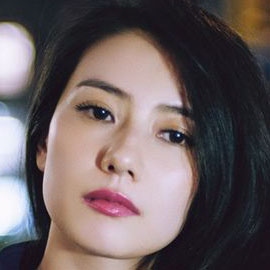
\includegraphics[width=0.8\textwidth]{./1/原始图.jpg}
        \end{minipage}
        }
        \subfigure[模版图]{
            \begin{minipage}[t]{0.3\linewidth}
            \centering
            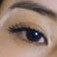
\includegraphics[width=0.2\textwidth]{./模版图.jpg}
        \end{minipage}
        }
        \subfigure[模板匹配结果]{
            \begin{minipage}[t]{0.3\linewidth}
            \centering
            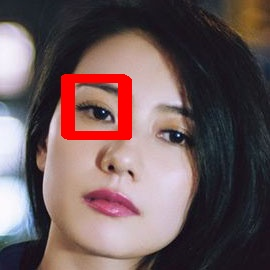
\includegraphics[width=0.8\textwidth]{./1/result.jpg}
            \end{minipage}
        }
        \centering
        \caption{模板匹配——单匹配结果}\label{fig:digit}
  \end{figure}


    \begin{figure}[htbp]
        \centering
        \subfigure[原图]{
            \begin{minipage}[t]{0.3\linewidth}
            \centering
            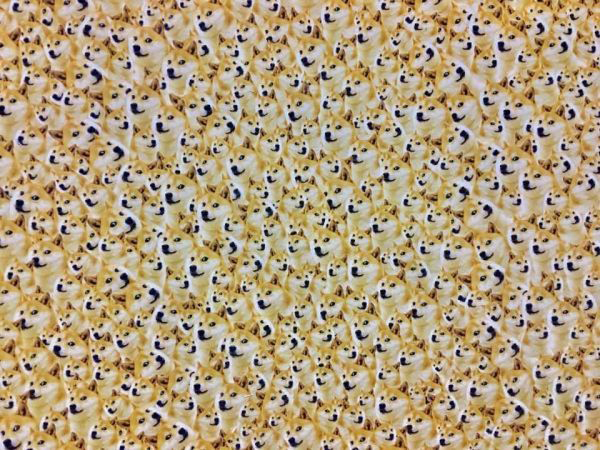
\includegraphics[width=0.8\textwidth]{./1/原始图2.jpg}
        \end{minipage}
        }
        \subfigure[模版图]{
            \begin{minipage}[t]{0.3\linewidth}
            \centering
            
\includegraphics[width=0.2\textwidth]{./模版图2.jpg}
        \end{minipage}
        }
        \subfigure[模板匹配结果]{
            \begin{minipage}[t]{0.3\linewidth}
            \centering
            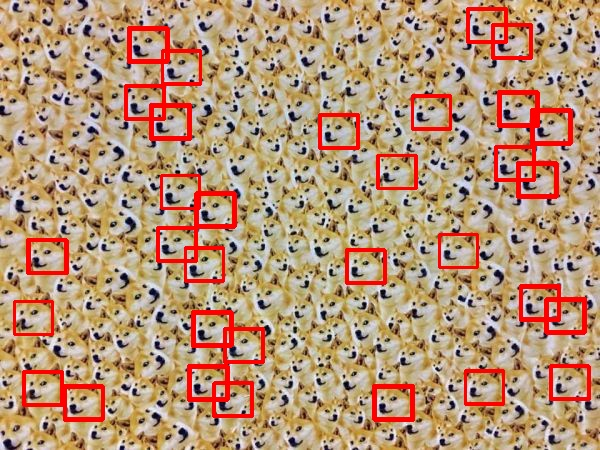
\includegraphics[width=0.8\textwidth]{./1/result2.jpg}
            \end{minipage}
        }
        \centering
        \caption{模板匹配——多匹配结果}\label{fig:digit}
  \end{figure}

  \newpage

\subsubsection*{彩色与纹理边缘检测}

    \begin{figure}[htbp]
        \centering
        \subfigure[彩色边缘检原图]{
            \begin{minipage}[t]{0.4\linewidth}
            \centering
            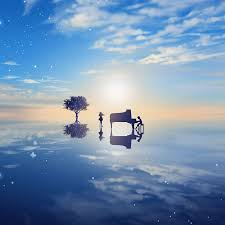
\includegraphics[width=0.6\textwidth]{./3/彩色图像.jpg}
        \end{minipage}
        }
        \subfigure[彩色边缘检结果]{
            \begin{minipage}[t]{0.4\linewidth}
            \centering
            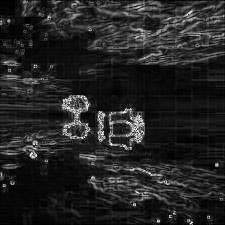
\includegraphics[width=0.6\textwidth]{./3/result_sobel_edge_detection_rgb.jpg}
            \end{minipage}
        }
        \subfigure[纹理边缘检测原图]{
            \begin{minipage}[t]{0.4\linewidth}
            \centering
            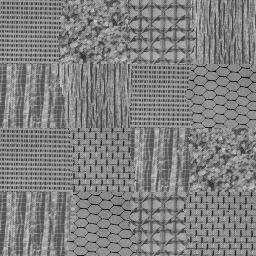
\includegraphics[width=0.6\textwidth]{./3/纹理图像.jpg}
        \end{minipage}
        }
        \subfigure[纹理边缘检测结果]{
            \begin{minipage}[t]{0.4\linewidth}
            \centering
            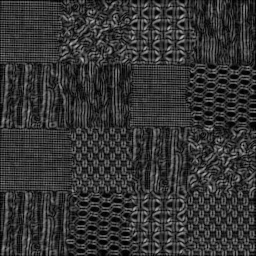
\includegraphics[width=0.6\textwidth]{./3/result_edge_detection_texture.jpg}
            \end{minipage}
        }
        \centering
        \caption{彩色与纹理边缘检测}\label{fig:digit}
  \end{figure}
  
\newpage
  
\subsection* {快速傅里叶变换}


    \begin{figure}[htbp]
        \centering
        \subfigure[原图]{
            \begin{minipage}[t]{0.4\linewidth}
            \centering
            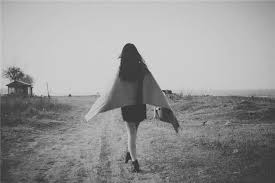
\includegraphics[width=0.8\textwidth]{./5/images.jpg}
        \end{minipage}
        }
        \subfigure[FFT 结果]{
            \begin{minipage}[t]{0.4\linewidth}
            \centering
            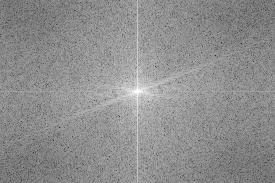
\includegraphics[width=0.8\textwidth]{./5/result.jpg}
            \end{minipage}
        }
        \centering
        \caption{傅里叶变换}\label{fig:digit}
  \end{figure}  
        
    \begin{figure}[htbp]
        \centering
        \subfigure[对 FFT 结果反 FFT 结果]{
            \begin{minipage}[t]{0.4\linewidth}
            \centering
            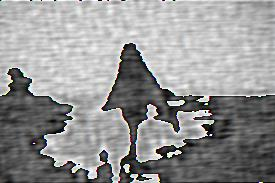
\includegraphics[width=0.8\textwidth]{./5/result2.jpg}
            \end{minipage}
        }
        \centering
        \caption{反傅里叶变换}\label{fig:digit}
  \end{figure}
  
\newpage

\subsubsection*{局部平均图像平滑}

      \begin{figure}[htbp]
        \centering
        \subfigure[原图]{
            \begin{minipage}[t]{0.4\linewidth}
            \centering
            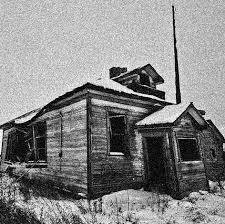
\includegraphics[width=0.6\textwidth]{./7/images.jpg}
        \end{minipage}
        }
        \subfigure[卷积核:$2\times 2$]{
            \begin{minipage}[t]{0.4\linewidth}
            \centering
            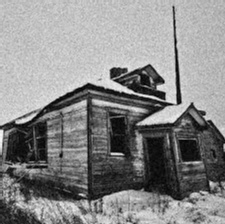
\includegraphics[width=0.6\textwidth]{./7/result——2X2.jpg}
            \end{minipage}
        }
        \subfigure[卷积核:$3\times 3$]{
            \begin{minipage}[t]{0.4\linewidth}
            \centering
            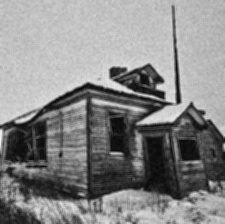
\includegraphics[width=0.6\textwidth]{./7/result——3X3.jpg}
            \end{minipage}
        }
        
        \subfigure[卷积核:$9\times 9$]{
            \begin{minipage}[t]{0.4\linewidth}
            \centering
            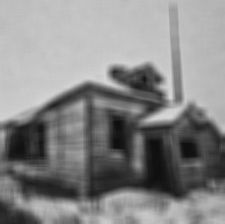
\includegraphics[width=0.6\textwidth]{./7/result——9X9.jpg}
            \end{minipage}
        }
        \centering
        \caption{局部平均}\label{fig:digit}
  \end{figure}

  
\subsection*{多帧平均图像平滑}

    \begin{figure}[htbp]
        \centering
        \subfigure[原图之一]{
            \begin{minipage}[t]{0.4\linewidth}
            \centering
            \includegraphics[width=0.6\textwidth]{./9/WechatIMG1.jpg}
        \end{minipage}
        }
        \subfigure[结果]{
            \begin{minipage}[t]{0.4\linewidth}
            \centering
            
\includegraphics[width=0.6\textwidth]{./9/result.jpg}
            \end{minipage}
        }
        \centering
        \caption{多帧平均}\label{fig:digit}
  \end{figure}
  
\newpage
  
\section{主要核心代码}

\paragraph{模板匹配}

\lstset{language=python}
\begin{lstlisting}
# encoding:utf-8
import cv2
import numpy as np

#加载原图
img = cv2.imread("原始图2.jpg")
#将原图转换成灰度图
img_gray = cv2.cvtColor(img, cv2.COLOR_BGR2GRAY)
#加载模版图
template = cv2.imread('模版图2.jpg',0)
#读取模版图的尺寸
w, h = template.shape[::-1]
#使用 matchTemplate 函数进行匹配
res = cv2.matchTemplate(img_gray,template,cv2.TM_CCOEFF_NORMED)
#设置阀值
threshold = 0.7
loc = np.where( res >= threshold)
#在原始图像上标记匹配区域
for x in zip(*loc[::-1]):
        cv2.rectangle(img, x, (x[0] + w, x[1] + h), (0,0,255), 2)
#显示图像
cv2.imwrite('result2.jpg', img, [int(cv2.IMWRITE_JPEG_QUALITY), 95])
\end{lstlisting}

\paragraph{彩色图像边缘检测}

\lstset{language=python}
\begin{lstlisting}
import numpy as np
import cv2
from matplotlib import pyplot

img = cv2.imread('彩色图像.jpg')
R, G, B = cv2.split(img)

# 分别对三个通道进行拉普拉斯边缘检测
lapR = cv2.Laplacian(R, cv2.CV_64F)
lapG = cv2.Laplacian(G, cv2.CV_64F)
lapB = cv2.Laplacian(B, cv2.CV_64F)
# 对 lap 取绝对值
lapR = np.uint8(np.absolute(lapR))
lapG = np.uint8(np.absolute(lapG))
lapB = np.uint8(np.absolute(lapB))
# 求三个通道的梯度
combined = np.sqrt(np.power(np.uint16(lapR), 2) + np.power(np.uint16(lapG), 2) + np.power(np.uint16(lapB), 2))
combined = np.uint8(combined)

cv2.imwrite('result_laplacian_edge_detection_rgb.jpg', combined, [int(cv2.IMWRITE_JPEG_QUALITY), 95])

# Sobel 算子
edge = []
for one in [R, G, B]:
	# x方向的梯度
	sobelX = cv2.Sobel(one, cv2.CV_64F, 1, 0)
	sobelX = np.uint8(np.absolute(sobelX))
	# y方向的梯度
	sobelY = cv2.Sobel(one, cv2.CV_64F, 0, 1)
	sobelY = np.uint8(np.absolute(sobelY))
	# 权重加和
	sobelCombined = cv2.addWeighted(sobelX, 0.4, sobelY, 0.4, 0)
	edge.append(sobelCombined)

combined = np.sqrt(np.power(np.uint16(edge[0]), 2) + np.power(np.uint16(edge[1]), 2) + np.power(np.uint16(edge[2]), 2))
cv2.imwrite('result_sobel_edge_detection_rgb.jpg', combined, [int(cv2.IMWRITE_JPEG_QUALITY), 95])
\end{lstlisting}

\paragraph{纹理边缘检测}

\lstset{language=python}
\begin{lstlisting}
import numpy as np
import cv2

img = cv2.imread('纹理图像.jpg', cv2.IMREAD_GRAYSCALE)

# 平均灰度值
MATRIX_SIZE = 3
kernel = np.ones((MATRIX_SIZE, MATRIX_SIZE), np.float) / (MATRIX_SIZE * MATRIX_SIZE)
img = cv2.filter2D(img, cv2.CV_64F, kernel)
# cv2.imwrite('pre.jpg', img, [int(cv2.IMWRITE_JPEG_QUALITY), 95])

# x方向的梯度
sobelX = cv2.Sobel(img, cv2.CV_64F, 1, 0)
sobelX = np.uint8(np.absolute(sobelX))
# y方向的梯度
sobelY = cv2.Sobel(img, cv2.CV_64F, 0, 1)
sobelY = np.uint8(np.absolute(sobelY))
# 权重加和
sobelCombined = cv2.addWeighted(sobelX, 0.5, sobelY, 0.5, 0)

# kernel = np.array([[0.125, 0.125, 0.125], [0.125, 0.125, 0.125],[0.125, 0.125, 0.125]])
# result = cv2.filter2D(sobelCombined, cv2.CV_64F, kernel)
cv2.imwrite('result_edge_detection_texture.jpg', sobelCombined, [int(cv2.IMWRITE_JPEG_QUALITY), 95])
\end{lstlisting}

\paragraph{快速傅里叶变换}

\lstset{language=python}
\begin{lstlisting}
# encoding:utf-8
import cv2
import numpy as np
from matplotlib import pyplot as plt

#加载原图
img = cv2.imread('images.jpg',0)
#进行傅立叶变换
dft = cv2.dft(np.float32(img),flags = cv2.DFT_COMPLEX_OUTPUT)
#将图像变换的原点移动到频域矩形的中心
dft_shift = np.fft.fftshift(dft)
#对傅立叶变换的结果进行对数变换
fft_log = 20*np.log(cv2.magnitude(dft_shift[:,:,0],dft_shift[:,:,1]))
#输出 fft 变换后的图像
cv2.imwrite('result.jpg', fft_log, [int(cv2.IMWRITE_JPEG_QUALITY), 95])
\end{lstlisting}

\lstset{language=python}
\begin{lstlisting}
# encoding:utf-8
import numpy as np
from PIL import Image
from numpy.fft import fft,ifft

#加载原图
img = Image.open('images.jpg')
img2 = np.fromstring(img.tobytes(),dtype = np.int8)
#设置阀值
threshold  =  90000
#傅里叶变换并滤除低频信号
result = fft(img2)
result = np.where(np.absolute(result) < threshold , 0 , result)
#傅里叶反变换,保留实部
result = ifft(result)
result = np.int8(np.real(result))
#转换为图像,并输出保存
im = Image.frombytes(img.mode,img.size,result)
im.save('result2.jpg')
\end{lstlisting}

\paragraph{局部平均图像平滑}

\lstset{language=python}
\begin{lstlisting}
# encoding:utf-8
import cv2
import numpy as np
import matplotlib.pyplot as plt
 
#加载原图
img = cv2.imread('images.jpg')
source = cv2.cvtColor(img, cv2.COLOR_BGR2RGB)
#设置核的大小(取平均值的区间)
threshold = 9
#局部均值滤波
result = cv2.blur(source, (threshold, threshold)) 
#输出局部均值滤波后的图像
cv2.imwrite('result——9X9.jpg', result, [int(cv2.IMWRITE_JPEG_QUALITY), 95])

\end{lstlisting}

\paragraph{多帧平均图像平滑}

\lstset{language=python}
\begin{lstlisting}
import cv2
import numpy as np

#加载第一张图片
tmp = cv2.imread('./images/WechatIMG1.jpg')
tmp =  tmp.astype(np.float32)
img = tmp
#对给定的 17 张图片求和
for i in range(2,16):
    file_name = './images/WechatIMG' + str(i) + '.jpg'
    tmp = cv2.imread(file_name)
    tmp =  tmp.astype(np.float32)
    img = tmp + img
#求平均值
img = img / 17
img = img.astype(np.uint8)
#输出并保存图片
cv2.imwrite('result.jpg',img)
\end{lstlisting}


\section{参考资料}

\begin{thebibliography}{99}

\bibitem{zhao1} opencv dev team.\\
{\bf OpenCV 2.4.13.7 documentation\\}
{\bf https://docs.opencv.org/2.4/index.html\\}

\bibitem{zhao2} Adrian Rosebrock.\\
{\bf Long exposure with OpenCV and Python\\}
{\bf https://www.pyimagesearch.com/2017/08/14/long-exposure-with-opencv-and-python/\\}

\bibitem{zhao3} xiatwhu (Nick name).\\
{\bf python 简单图像处理(15) 图像的傅立叶变换\\}
{\bf https://www.cnblogs.com/xianglan/archive/2010/12/30/1922386.html\\}

\end{thebibliography}


\end{document}
